\documentclass{article}

\usepackage[T1]{fontenc}
\usepackage[utf8]{inputenc}
\usepackage[brazilian]{babel}
\usepackage{graphicx}
\usepackage[export]{adjustbox}[2011/08/13]
\usepackage{float}
\usepackage[pdftex]{hyperref}
\usepackage{epstopdf}
\usepackage{etoolbox}
\usepackage{amsmath}
\usepackage{amsfonts}
\usepackage{amssymb}
\usepackage{caption}
\usepackage{subcaption}
\usepackage{setspace}
\usepackage{tikz}
\usepackage{listings}
\usepackage{xcolor} 

\patchcmd{\thebibliography}{\section*}{\section}{}{}
\newcommand{\R}{\ensuremath{\mathbb{R}}}
\newcommand{\Prob}{\ensuremath{\mathbb{P}}}
\newcommand{\K}{\ensuremath{\mathbb{K}}}
\newcommand{\U}{\ensuremath{\mathbb{U}}}
\newcommand{\N}{\ensuremath{\mathbb{N}}}
\newcommand{\Lg}{\ensuremath{\mathbb{L}}}
\newcommand{\T}{\ensuremath{\rm Tr}}
\newcommand{\sg}{{\sigma(x_k)}}

\newcommand{\G}{\ensuremath{\mathcal{G}}}
\newcommand{\F}{\ensuremath{\mathcal{F}}}
\newcommand{\C}{\ensuremath{\mathcal{C}}}
\newcommand{\E}{\ensuremath{\mathcal{E}}}
\newcommand{\Hn}{\ensuremath{\mathcal{H}}}
%\newcommand{\Hoo}{\ensuremath{\mathcal{H}_\infty}}
\newcommand{\Hop}{\ensuremath{\mathcal{H}_{op}}}
% --------------------------------------------------
\newtheorem{theo}{Teorema}
\newtheorem{exa}{Exemplo}
\newtheorem{lemm}{Lema}
\newtheorem{coro}{Corolário}
\newtheorem{defn}{Definição}[section]

%opening
\lstset{ %
	backgroundcolor=\color{white},   % choose the background color; you must add \usepackage{color} or \usepackage{xcolor}
	basicstyle=\fontsize{8}{10}\ttfamily\color{black},        % the size of the fonts that are used for the code
	breakatwhitespace=true,         % sets if automatic breaks should only happen at whitespace
	breaklines=true,                 % sets automatic line breaking
	captionpos=t,                    % sets the caption-position to bottom
	commentstyle=\color{green},    % comment style
	extendedchars=true,              % lets you use non-ASCII characters; for 8-bits encodings only, does not work with UTF-8
	frame=tb,                    % adds a frame around the code
	keepspaces=true,                 % keeps spaces in text, useful for keeping indentation of code (possibly needs columns=flexible)
	keywordstyle=\color{cyan},       % keyword style
	language=C,                 % the language of the code
	numbers=left,                    % where to put the line-numbers; possible values are (none, left, right)
	numbersep=5pt,                   % how far the line-numbers are from the code
	numberstyle=\tiny\color{black}, % the style that is used for the line-numbers
	rulecolor=\color{gray},         % if not set, the frame-color may be changed on line-breaks within not-black text (e.g. comments (green here))
	showspaces=false,                % show spaces everywhere adding particular underscores; it overrides 'showstringspaces'
	showstringspaces=false,          % underline spaces within strings only
	showtabs=false,                  % show tabs within strings adding particular underscores
	stepnumber=1,                    % the step between two line-numbers. If it's 1, each line will be numbered
	stringstyle=\color{red},     % string literal style
	tabsize=2,                       % sets default tabsize to 2 spaces
}

\makeatletter
\def\code{\@ifnextchar[{\@with}{\@without}}%
\def\@with[#1]#2{%
}
\def\@without#1{%
	\subsection{\protect\detokenize{#1}}%
	\lstinputlisting[language=C, linewidth=1.3\linewidth]{#1}%
	\pagebreak%
}
\makeatother

\begin{document}

\begin{titlepage}
\begin{center}

\newcommand{\HRule}{\rule{\linewidth}{0.5mm}}
% Upper part of the page. The '~' is needed because \\
% only works if a paragraph has started.

\includegraphics[width=0.15\textwidth]{logoUnicamp}~\\[1cm]

\textsc{\LARGE Universidade Estadual de Campinas}\\[1.5cm]

\textsc{\Large Faculdade de Engenharia Mecânica}\\[0.5cm]

% Title
\HRule \\[0.4cm]
{ \huge \bfseries ES670 - Projeto de Sistemas Embarcados\\ \vspace{1cm} Relatório - Projeto Prático Parte 3\\
\Large{Requisito 3: Display LCD} \\[0.4cm] }

\HRule \\[1.5cm]

% Author and supervisor
\begin{minipage}{0.6\textwidth}
\begin{flushleft} \large
\emph{Nome:}\\
Daniel Dello Russo Oliveira\\Davi Rodrigues
\end{flushleft}
\end{minipage}
\begin{minipage}{0.2\textwidth}
\begin{flushright} \large
\emph{RA}\\ 101918\\116581
\end{flushright}
\end{minipage}

\vfill

% Bottom of the page
{\large \today}

\end{center}
\end{titlepage}


\onehalfspacing
\section{Objetivo} 
O objetivo do projeto é, de maneira incremental, implementar no \textit{target} os requisitos apresentados no roteiro\cite{bb:roteiro} inicialmente desenvolvendo o modelo e depois implementando cada requisito. Estes requisitos são referentes à configuração e implementação de entradas de teclado, acionamento de LEDs, \textit{display} de sete segmentos, protocolo de comunicação, \textit{display LCD}, medição de velocidade de rotação, \textit{PWM}, \textit{ADC} e Controlador. 
	
\section{Modelagem}
% Diagramas requisitos implementados, digrama de blocos, etc
Utilizando o Rational Rhapsody Modeler e tomando como base os requisitos propostos mostrados na figura \ref{fig:requisitos}, complementamos o modelo inicial\cite{bb:modelo} (requisitos de teclado e LEDs) adicionando um bloco ao modelo referente aos \textit{displays} de sete segmentos (REQ1C), conforme mostrado na figura \ref{fig:blocos}. Adicionamos também alguns blocos auxiliares relacionados ao gerenciamento de pinos \textit{GPIO} e a interrupções periódicas, que foram utilizados para nossa implementação do \textit{display} de sete segmentos e do \textit{buzzer}. Ao tratar o gerenciamento do \textit{display} e do \textit{buzzer} através de interrupções, livramos a \textit{thread} principal para que essa lide com outros problemas sem precisar se preocupar com a atualização periódica dos \textit{displays}.

Continuamos a complementar nosso diagrama adicionando um bloco responsável pela comunicação serial e um pela interpretação dos comandos referentes ao protocolo do requisito REQ2.

\begin{figure}[H]
	\centering
	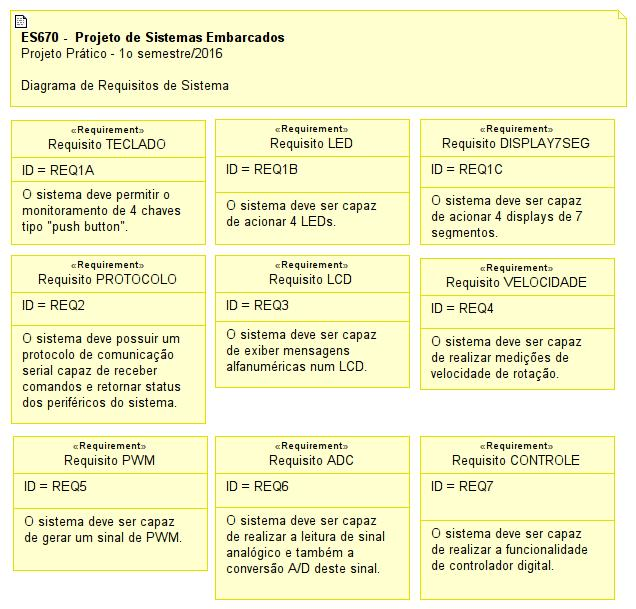
\includegraphics[width=0.9\linewidth]{requisitos}
	\caption{Diagrama de requisitos}
	\label{fig:requisitos}
\end{figure}
\begin{figure}[H]
	\centering
	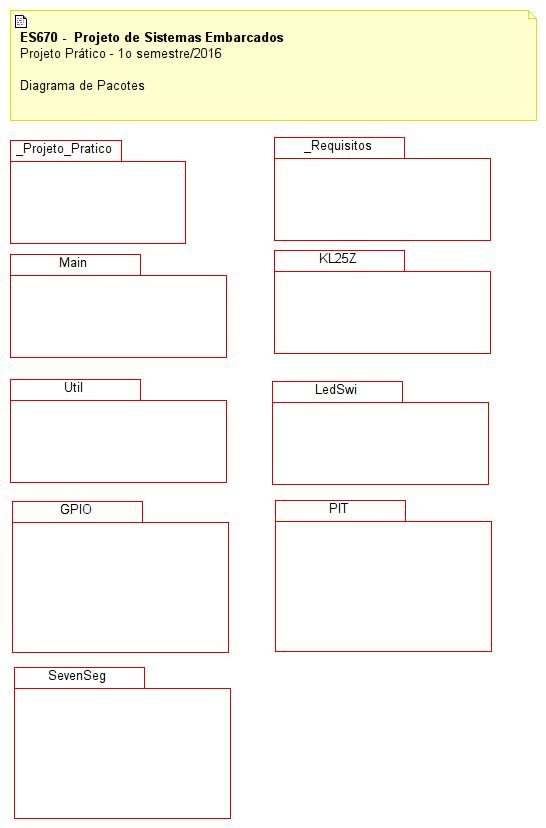
\includegraphics[width=0.9\linewidth]{pacotes}
	\caption{Diagrama de pacotes}
	\label{fig:pacotes}
\end{figure}
\begin{figure}[H]
	\centering
	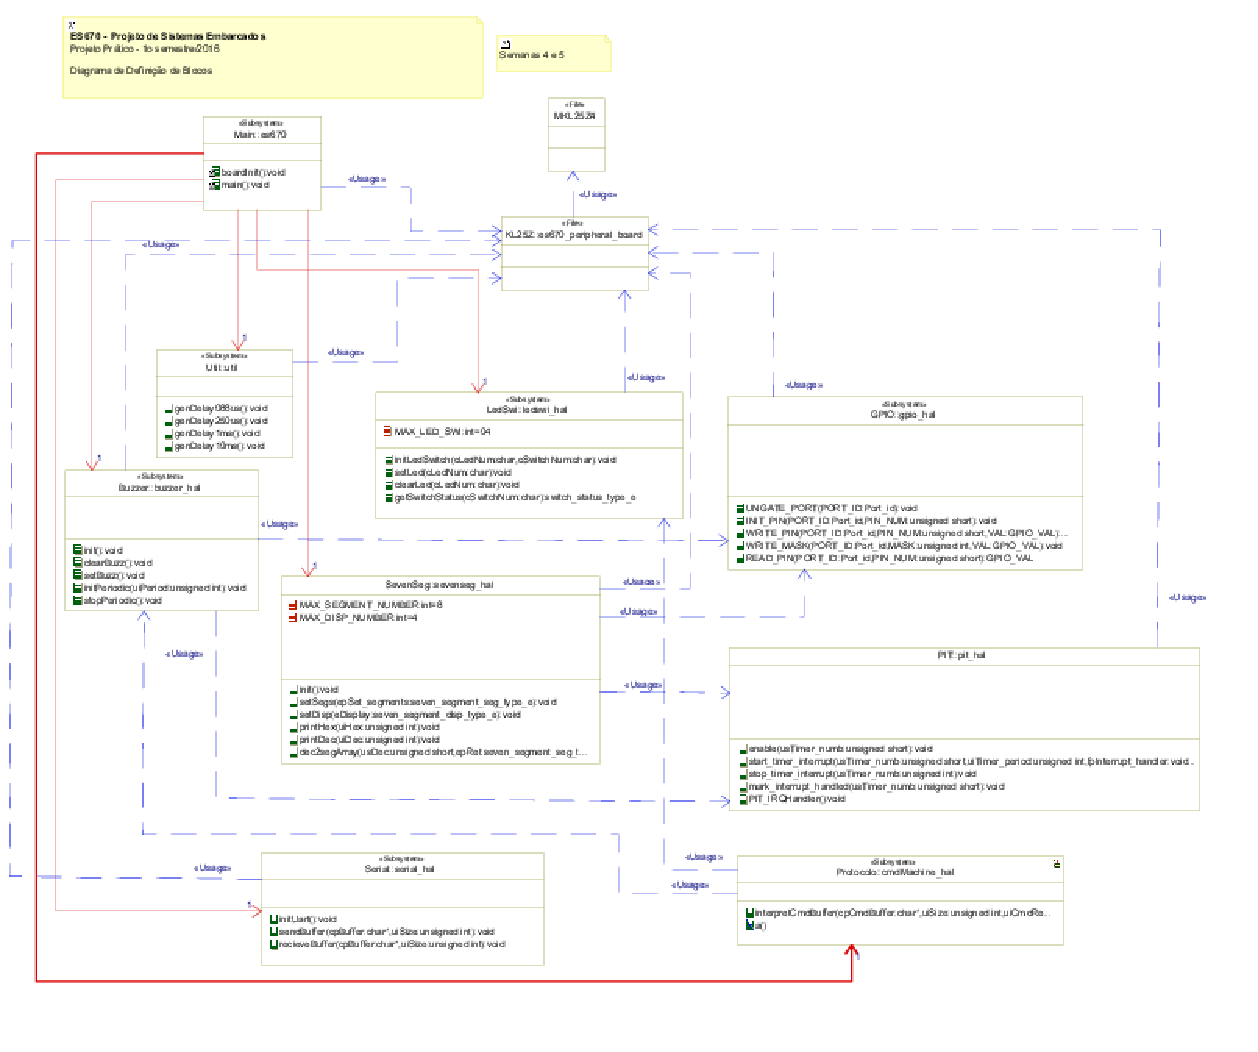
\includegraphics[width=1.5\linewidth, center]{blocos}
	\caption{Diagrama de definição de blocos}
	\label{fig:blocos}
\end{figure}

O bloco de \textit{GPIO\_hal} tem operações para desbloquear o \textit{clock} para uma porta, inicializar um pino em uma dada direção, escrever em um pino, escrever em um conjunto de pinos da mesma porta, ler a entrada em um pino e ler o valor de saída que está sendo controlado em um pino.

O bloco \textit{pit\_hal} tem tem operações para inicializar o \textit{PIT}, criar interrupções periódicas em um dos dois \textit{timers} disponíveis, desativar as interrupções em um \textit{timer} e marcar uma interrupção como tratada (deve ser feito pelos tratamentos de interrupção). Além disso esse bloco tem mais uma operação chamada \textit{PIT\_IRQHandler }que trata as interrupções do \textit{PIT}, essa operação precisa ser visível para o \textit{linker}, mas não deve ser chamada pelo usuário. É importante ressaltar que o \textit{clock} do \textit{PIT} é o \textit{bus\_clock} que no nosso caso é de $20MHz$

As operações do bloco \textit{sevenseg\_hal} cobrem a inicialização dos \textit{displays}, seleção manual de quais segmentos estarão ativos (feita através da passagem de um vetor com os segmentos desejados), ativação manual de um dos \textit{displays} (desativando todos os outros), conversão de dígito hexadecimal ou decimal em vetor de segmentos (para ser passado para a função de seleção de segmentos) e impressão automática de um valor hexadecimal ou decimal através das interrupções de \textit{timer}.

O bloco do \textit{buzzer\_hal} também ganhou duas novas operações, uma para criar uma onda quadrada no \textit{buzzer} com um certo período (e \textit{duty cycle} de $50\%$), através de interrupções de \textit{timer}, e outra para remover essa onda.

O bloco \textit{ledswi\_hal} foi alterado para lidar melhor com a inicialização separada dos pinos como Led e Switch e também foi adicionada uma função para ler o estado atual de um pino configurado como LED.

O bloco \textit{serial\_hal} é responsável pela configuração da UART para comunicação serial e pelo envio de recebimento de dados através desse protocolo.

O bloco \textit{cmdMachine\_hal} lida com a interpretação dos comandos e geração da string de resposta. Em nossa implementação, escolhemos tratar uma string já bufferada de commandos ao invés de trabalhar caractere a caractere. A máquina de estados do tratamento dos comandos pode ser vista na figura \ref{fig:estados}.

\begin{figure}[H]
	\centering
	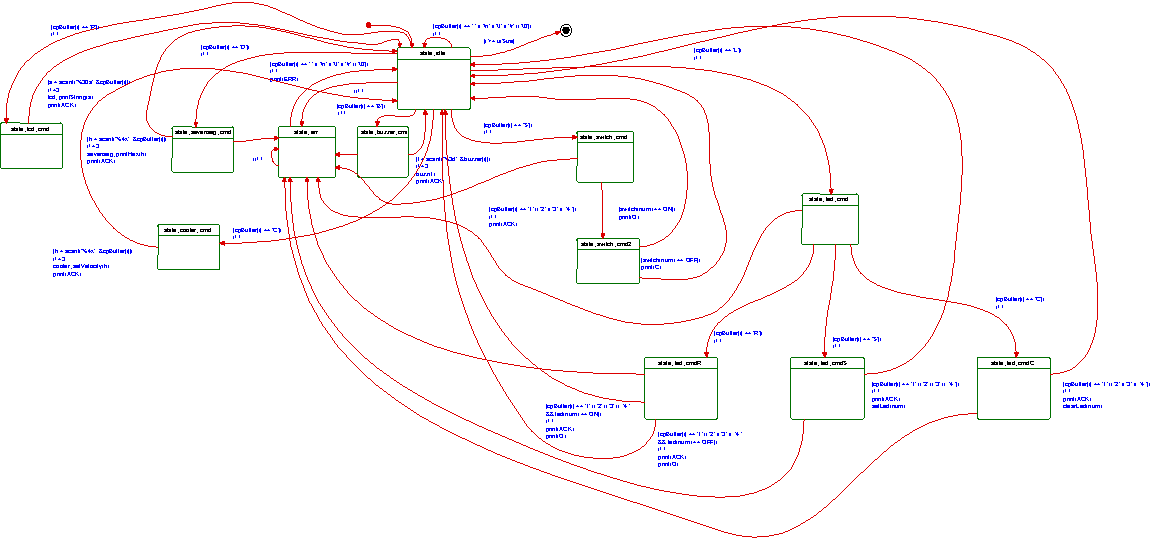
\includegraphics[width=1.5\linewidth, center]{estados}
	\caption{Diagrama de máquina de estados para interpretação dos comandos}
	\label{fig:estados}
\end{figure}

A máquina de estados recebe um buffer de caracteres por vez, e avalia caracter a caracter percorrendo o buffer. Após cada ação a máquina retorna para o estado "state\_idle" para a avaliação da próxima ação do buffer de dados. Sempre que a máquina de estados encontra um caractere inesperado ou sem significado, ela entra no estado "state\_err", retornando um erro e descartando todos caracteres até encontrar o próximo espaço em branco. Os outros estados são acionados através dos seguintes caracteres: 'B' para buzzer, 'S' para switch e 'L' para led.
No caso do buzzer,  após interpretar o caracter 'B', a máquina espera ler três caracteres numéricos que correspondem ao tempo em que o buzzer permanecerá ativo, retornando para o estado 'statez\_idle' após, para avaliar a próxima ação do buffer de entrada.
Para o switch, após a leitura de 'S', a máquina de estados espera a leitura de um caractere numérico, de 1 a 4, que corresponde de qual switch faremos a leitura. Recebemos como retorno 'O' caso o switch esteje acionado, e 'C' caso contrário.
No caso do led, após a leitura de 'L' a máquina de estado espera mais um caractere indicando a ação desejada. Este caractere pode ser 'S' no caso de set, 'R' para read e 'C' para clear. Para todos estes casos, a máquina de estados esperará um caractere numérico indicando em qual dos leds a ação deverá ser executada.
Após cada ação executada com sucesso, o sistema responderá com 'ACK'.

\section{Diagramas Esquemáticos}
% Diagramas esquemáticos do target utilizados

\begin{figure}[H]
	\centering
	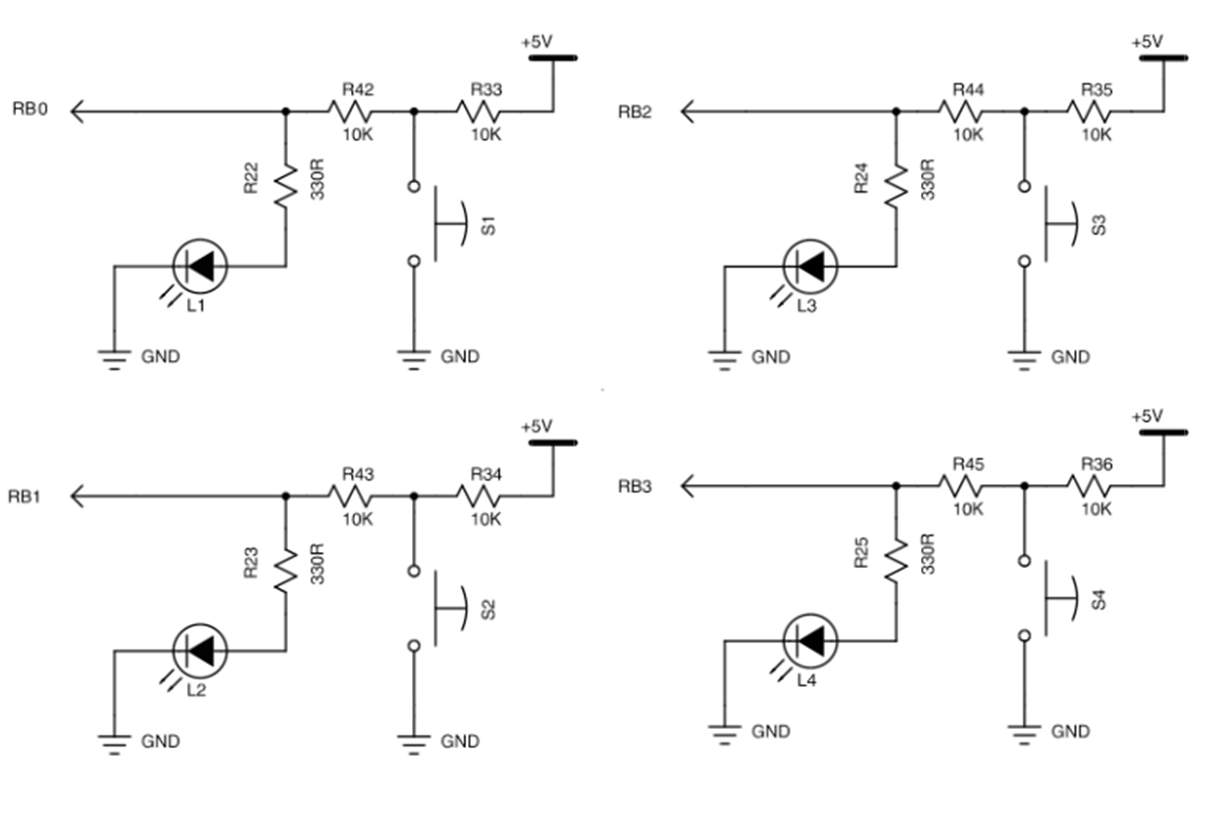
\includegraphics[width=0.7\linewidth]{esq_ledswi}
	\caption{Esquema teclado e LEDs}
	\label{fig:esq_ledswi}
\end{figure}
\begin{figure}[H]
	\centering
	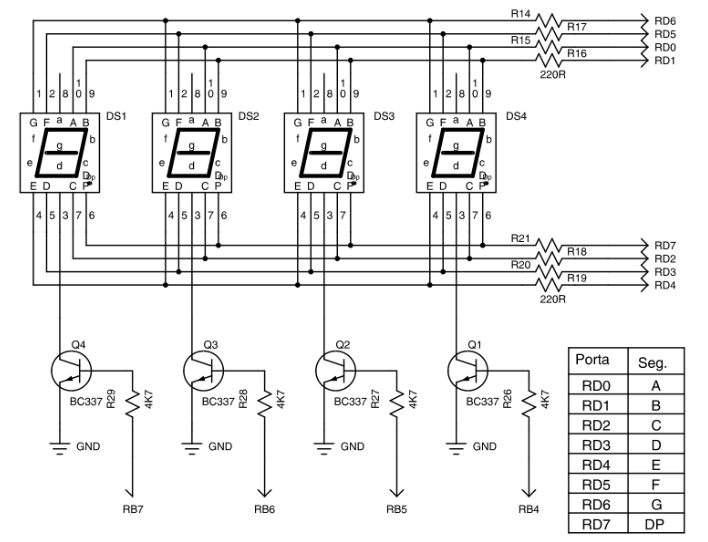
\includegraphics[width=0.9\linewidth]{esq_7seg}
	\caption{Esquema sete segmentos}
	\label{fig:esq_7seg}
\end{figure}
\begin{figure}[H]
	\centering
	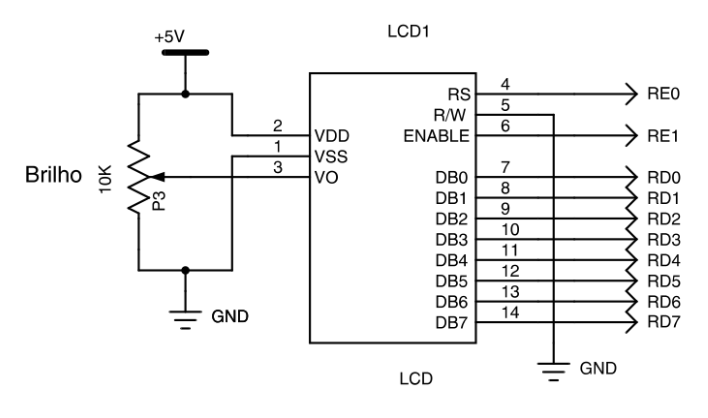
\includegraphics[width=0.9\linewidth]{esq_lcd}
	\caption{Esquema display LCD}
	\label{fig:esq_lcd}
\end{figure}

Os pinos apresentados acima, devem ser mapeados para os da placa \textit{FRDM-KL25Z} através do mapeamento apresentado na figura \ref{fig:pinout}
\begin{figure}[H]
	\centering
	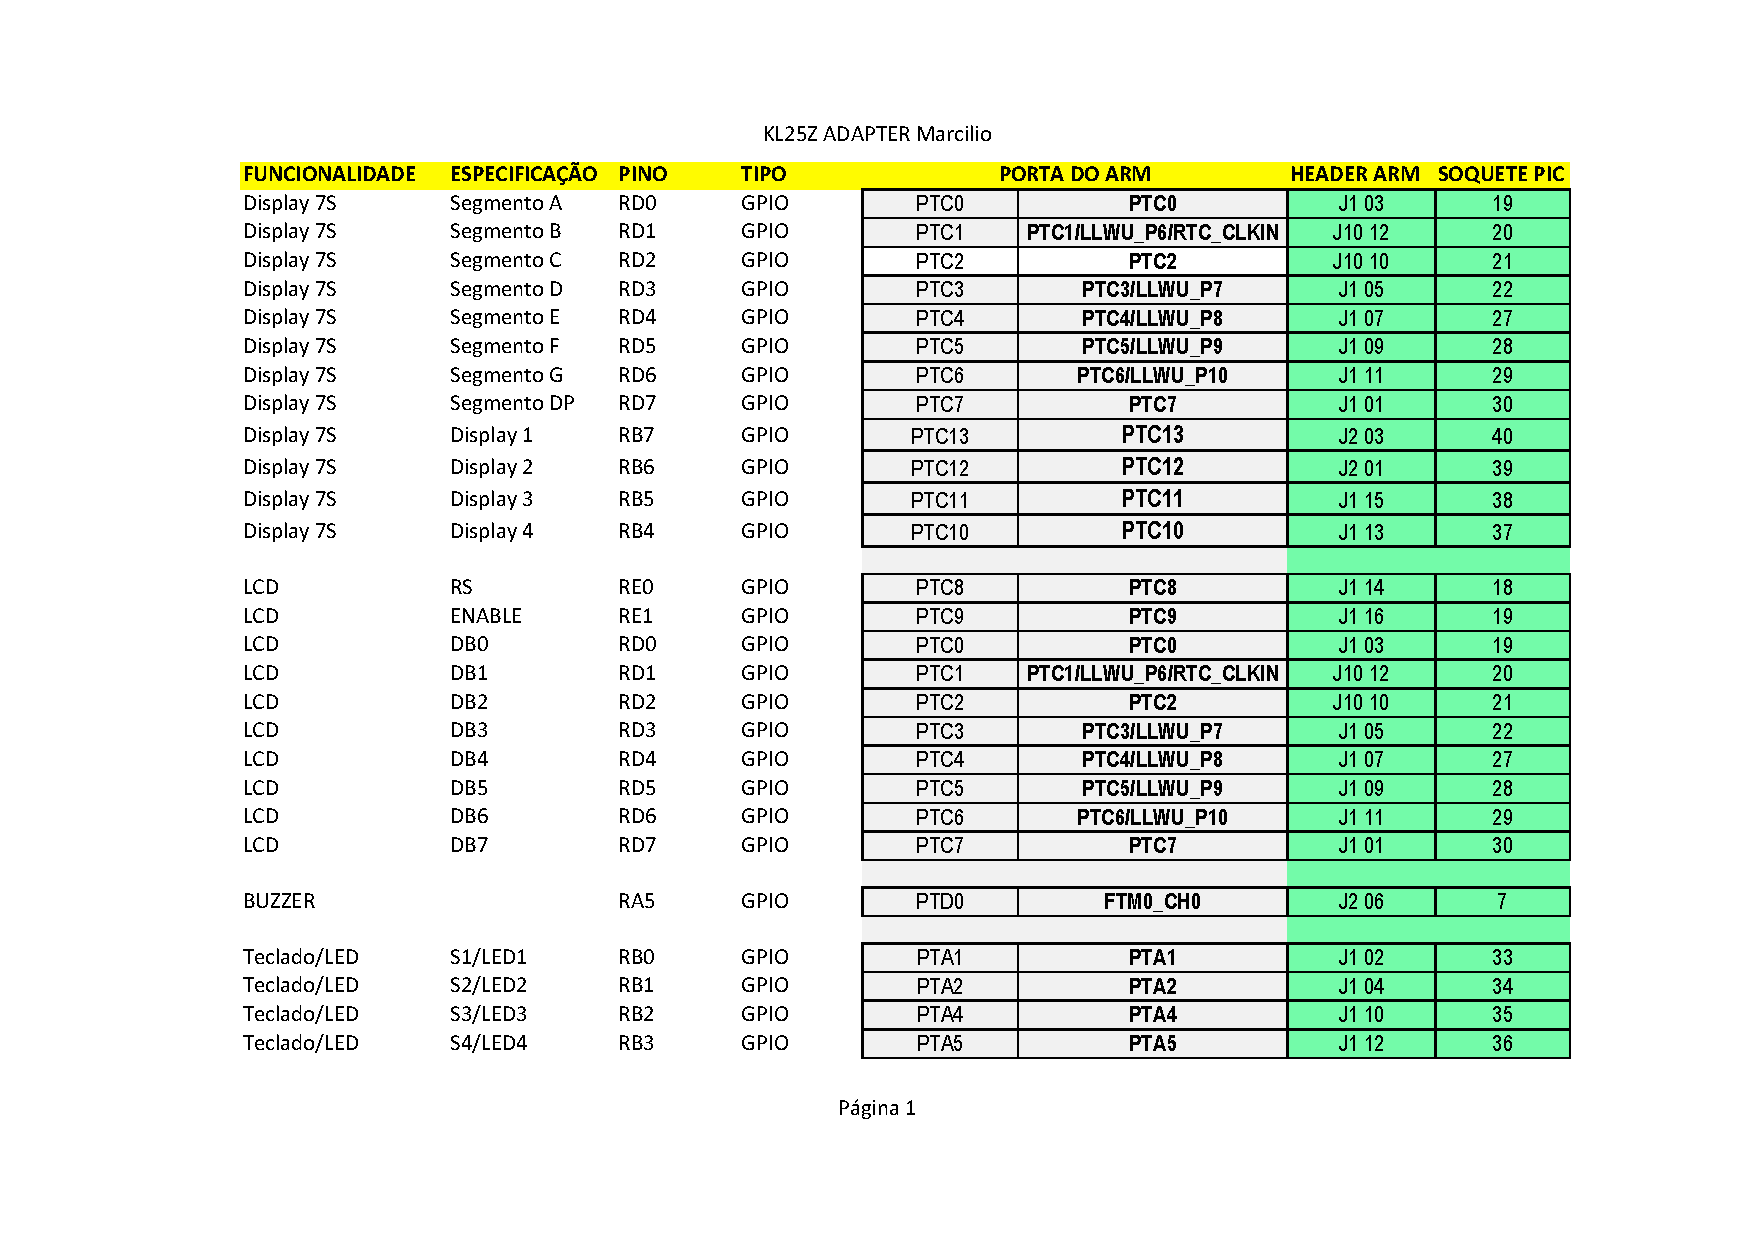
\includegraphics[width=0.9\linewidth]{Pinout}
	\caption{Mapeamento entre pinos dos esquemáticos e da placa FRDM-KL25Z}
	\label{fig:pinout}
\end{figure}

Como pode ser visto na figura \ref{fig:esq_7seg}, é necessário fazer um gerenciamento dos pinos PTC0 a PTC7 para selecionar os segmentos que serão ativados e PTC10 a PTC13 para selecionar quais \textit{displays} estarão ativos. Para isso, é preciso alternar qual \textit{display} está ativo e fazer a mudança nos segmentos para que cada \textit{display} esteja mostrando um valor diferente. É importante lembrar que a frequência dessa alternância seja escolhida de modo que o olho humano não perceba que os \textit{displays} estão ligando e desligando. Afim de garantir que essa alternância funcionará apropriadamente nós utilizamos o módulo \textit{PIT} para gerar uma interrupção a cada $3.125 ms$, conforme sugerido na aula 6 \cite{bb:aula6}. 


\section{Matriz de Rastreabilidade}
% Matriz de rastreabilidade de requisitos vs implementações
A matriz de rastreabilidade apresentada na tabela \ref*{tab:rastreabilidade} relaciona cada um dos requisitos com a sua implementação.
\begin{table}[H]
	\centering
	\caption{Matriz de Rastreabilidade}
	\label{tab:rastreabilidade}
	\small
	\scalebox{0.8}{
	\begin{tabular}{|c|l|}
		\hline \bfseries{ID do Requisito} & \bfseries{Implementação}\\ 
		\hline REQ1A 	& \texttt{ledswi\_hal.c}\\ 
						& \texttt{- void ledswi\_initLedSwitch(char cLedNum, char cSwitchNum)}\\
						& \texttt{- switch\_status\_type\_e ledswi\_getSwitchStatus(char cSwitchNum)}\\
						& \texttt{- void ledswi\_initSwich(ledswi\_pin\_type\_e ePin)}\\
		\hline REQ1B 	& \texttt{ledswi\_hal.c}\\ 
						& \texttt{- void ledswi\_initLedSwitch(char cLedNum, char cSwitchNum)}\\
						& \texttt{- void ledswi\_setLed(char cLedNum)}\\ 
						& \texttt{- void ledswi\_clearLed(char cLedNum)}\\
						& \texttt{- void ledswi\_initLed(ledswi\_pin\_type\_e ePin)}\\
						& \texttt{- led\_status\_type\_e ledswi\_getLedStatus(ledswi\_pin\_type\_e eLedPin)}\\
		\hline REQ1C 	& \texttt{sevenseg\_hal.c}\\ 
						& \texttt{- void sevenseg\_init(void)}\\
						& \texttt{- void sevenseg\_setSegs(seven\_segment\_seg\_type\_e* epSet\_segments)}\\
						& \texttt{- void sevenseg\_setDisp(seven\_segment\_disp\_type\_e eDisplay)}\\
						& \texttt{- void sevenseg\_printDec(unsigned int uiDec)}\\
						& \texttt{- void sevenseg\_printHex(unsigned int uiHex)}\\
		\hline REQ2 	& \texttt{serial\_hal.c}\\ 
						& \texttt{- void serial\_initUart(void)}\\
						& \texttt{- void serial\_sendBuffer(char *cpBuffer, unsigned int uiSize)}\\
						& \texttt{- int serial\_recieveBuffer(char *cpBuffer, unsigned int uiSize)}\\
						& \texttt{cmdMachine\_hal.c}\\
						& \texttt{- void cmdmachine\_interpretCmdBuffer(char *cpCmdBuffer, unsigned int uiSize, char* cpCmdRes)}\\
						& \texttt{- int handleError(char *cpCmdBuffer, unsigned int uiSize, char* cpCmdRes)}\\
						& \texttt{- int handleBuzzer(char *cpCmdBuffer, unsigned int uiSize, char* cpCmdRes)};\\
						& \texttt{-int getBuzzMs(char *cpCmdBuffer)}\\
						& \texttt{-unsigned int handleSwitch(char *cpCmdBuffer, unsigned int uiSize, char* cpCmdRes)}\\
						& \texttt{-unsigned int handleLed(char *cpCmdBuffer, unsigned int uiSize, char* cpCmdRes)}\\
						& \texttt{-ledswi\_pin\_type\_e parseLedNum(char cLedInput)}\\
						& \texttt{-unsigned int handleIdle(char *cpCmdBuffer, unsigned int uiSize, char* cpCmdRes)}\\
		\hline 
	\end{tabular}
	} 
	\normalsize
\end{table}
\section{Notas}
% Dificuldades, observações relevantes, correções, ...
\subsection{LCD e interrupções}
Para escrever no LCD precisamos gerar um pulso no seu pino de enable. Para garantir que esse pulso terá a duração certa, foi precisamos mascarar as interrupções durante esse pulso. Como as interrupções do display tem um período de aproximadamente 3ms e o pulso do LCD tem a mesma duração encontramos várias dificuldades ao controlar os dois sem mascarar as interrupções pela duração do pulso.

\subsection{Leitura do Estado dos LEDs}
Como uma extensão ao protocolo proposto no roteiro \cite{bb:roteiro}, acrescentamos o comando \textit{LRd} onde $d$ é um digito de 1 a 4, que nos retorna o estado atual do LED referenciado. Para recuperar esse estado devemos saber qual valor está sendo controlado para um pino de saída digital, o que é feito lendo o registrador GPIOx\_PDOR.

\subsection{Interrupções do Buzzer e mudança de Baud Rate}
Ao utilizar interrupções para cuidar do acionamento e controle do Buzzer, conseguímos executar essa funcionalidade de maneira assíncrona, garantindo que essa funcionalidade não vai interferir com ou ser interferida pelas outras. Isso é notavelmente importante com a comunicação serial, uma vez que a velocidade de leitura é crítica e se essa for alterada, corremos o risco de perder informações ou alterar o tempo de execução de nosso ciclo.

\subsection{Bufferização dos comandos}
Para diminuir a chance de perder informações que são enviadas por serial, escolhemos ler uma série de caracteres e armazená-los em um buffer antes de interpretá-los, ao invés de ler e interpretar caractere a caractere. Interrompemos esse processo de leitura no caso de buffer overflow ou quando encontramos uma quebra de linha. Interpretar uma série de comandos bufferizados introduziu uma dificuldade extra ao projeto, pois agora nossa máquina de estados tem que levar em consideração que um comando pode estar errado e o próximo não, logo o primeiro deve ser ignorado e o segundo executado.

\subsection{Gerenciamento de GPIO e macros}
Detectamos logo no início do projeto um defeito estrutural no código fornecido quando lidando com GPIO: o identificador da porta e o número do pino utilizado eram referenciados em diversos locais diferentes do código dificultando de maneira agravante mudanças na configuração de hardware. Para resolver isso inicialmente pensamos em utilizar o arquivo \textit{fsl\_gpio\_hal.h} da biblioteca da \textit{FRDM-Kl25Z}, mas isso não nos foi permitido. Como calcular as posições na memória de cada registrador seria reimplementar a biblioteca, escolhemos por criar macros que geram o mesmo estilo de código utilizado no exemplo fornecido através do operador de concatenação (\#\#) do pré processador. Esse operador apresenta algumas particularidades, a principal sendo que macros que o utilizam em seu corpo não tem seus argumentos expandidos \cite{bb:preprocessor}. Para circular essa dificuldade criamos uma outras macros que funcionam como uma \textit{wrappers} para essas macros, fazendo assim que seus argumentos sejam expandidos antes da chamada da concatenação. 

As macros que fazem a concatenação propriamente ditas não devem ser chamadas pelo usuário (sendo identificadas por um \_ no início de seus nomes).

Outra dificuldade relacionada a esse módulo é que a expansão dos argumentos das macros não para quando chega em alguma \textit{token} não definida, no caso o identificador das portas (A,B,C,D,E). Para contornar esse problema utilizamos \textit{typedefs} para definir esses identificadores como \textit{tokens} válidas.

\subsection{Interrupções por timer}
Outro problema que enfrentamos foi com a implementação das interrupções por timer através do PIT, notavelmente pela dificuldade de encontrar uma documentação clara sobre o NVIC e pois a documentação fornecida para o PIT inverte a endianness dos registradores em relação aos registradores de GPIO.

\subsection{Leitura de entradas digitais}
Nesse laboratório tivemos dificuldades relacionadas à leitura do estado dos botões. O problema encontrado ocorreu pois quando o desbloqueamos o \textit{clock} para uma porta do controlador no código fornecido estávamos desabilitando o \textit{clock} para todas as outras portas. Como o \textit{clock} só afeta significativamente os pinos configurados como \textit{input}, se o módulo \textit{ledswi\_hal} fosse inicializado por último (como é feito no código do professor) o problema não seria notado.

\subsection{Estilo de Documentação}
Não conseguimos nos adaptar ao estilo de comentários sugerido pelo professor, que nos parece introduzir uma quantidade desnecessária de burocracia. Formatar todos os comentários para caber dentro daquele quadrado tomava mais tempo que o planejamento e a implementação do código e muita informação redundante estava sendo inserida (bastava ler a interface da função para saber seu nome e o tipo de seus argumentos). Escolhemos substituir todos os comentários do código pelo padrão \textit{javadoc}, com o qual estamos mais familiarizados, que é capaz de documentar de maneira eficiente o código.

\subsection{Outros}
Também tivemos dificuldades com a instalação do \textit{Rhapsody Rational Modeler} no \textit{Linux} (através do \textit{Wine}), pois ele necessita da instalação das seguintes dlls nativas do \textit{Windows}: \textit{comctl32}, \textit{msvcirt} e \textit{riched20}.\\

 É relevante lembrar de utilizar o modificador \textit{volatile} para variáveis que serão modificadas durante o tratamento de interrupções, dessa maneira o otimizador sabe que não deve alterar comandos que envolvem essa variável.
 

\begin{thebibliography}{widestlabel}
	\bibitem{bb:roteiro}{Roteiro de Laboratório - Semanas 04 e 05 (disponibilizado para os alunos)}
	\bibitem{bb:modelo}{Projeto do Modelo Inicial do Sistema (disponibilizado para os alunos)}
	\bibitem{bb:codigo}{Código Fonte Inicial em Linguagem C (disponibilizado para os alunos)}
	\bibitem{bb:aula6}{Notas de Aula - Semanas 06 (disponibilizado para os alunos)}
	\bibitem{bb:preprocessor}{The C Preprocessor (Concatenation) \url{https://gcc.gnu.org/onlinedocs/cpp/Concatenation.html#Concatenation}}
\end{thebibliography}
\pagebreak
\section{Apêndice}
% Colocar como apêndice toda a listagem do código fonte
Listagem dos códigos fonte:
\code{../Sources/Buzzer/buzzer_hal.c}
\code{../Sources/Buzzer/buzzer_hal.h}
\code{../Sources/fsl_debug_console.c}
\code{../Sources/GPIO/gpio_hal.h}
\code{../Sources/KL25Z/es670_peripheral_board.h}
\code{../Sources/LCD/lcd_hal.c}
\code{../Sources/LCD/lcd_hal.h}
\code{../Sources/LedSwi/ledswi_hal.c}
\code{../Sources/LedSwi/ledswi_hal.h}
\code{../Sources/Main/es670.c}
\code{../Sources/Mcg/mcg_hal.c}
\code{../Sources/Mcg/mcg_hal.h}
\code{../Sources/PIT/pit_hal.c}
\code{../Sources/PIT/pit_hal.h}
\code{../Sources/print_scan.c}
\code{../Sources/print_scan.h}
\code{../Sources/Protocolo/cmdmachine_hal.c}
\code{../Sources/Protocolo/cmdmachine_hal.h}
\code{../Sources/Serial/serial_hal.c}
\code{../Sources/Serial/serial_hal.h}
\code{../Sources/SevenSeg/sevenseg_hal.c}
\code{../Sources/SevenSeg/sevenseg_hal.h}
\code{../Sources/Util/util.c}
\code{../Sources/Util/util.h}
\end{document}

